% ============================================================
%  ECE569 — Homework 4: Histogram Generation
%  Author : Joel Maldonado  |  University of Arizona
%  Workflow:
%    1. sbatch run_exp1.slurm && sbatch run_exp2.slurm  (from build_dir on HPC)
%    2. git pull  (to get output files locally)
%    3. cd ece569/labs/hw4/report
%    4. python3 parse_times.py --inject hw4_report.tex
%    5. pdflatex hw4_report.tex
% ============================================================
\documentclass[11pt, letterpaper]{article}

\usepackage[margin=1in]{geometry}
\usepackage{booktabs}
\usepackage{array}
\usepackage{amsmath}
\usepackage{amssymb}
\usepackage{listings}
\usepackage{xcolor}
\usepackage{hyperref}
\usepackage{caption}
\usepackage{subcaption}
\usepackage{float}
\usepackage{parskip}
\usepackage{enumitem}
\usepackage{fancyhdr}
\usepackage{graphicx}

% figures are in build_dir/Histogram_output/figures/, relative to this file
\graphicspath{{../../../build_dir/Histogram_output/figures/}}

\pagestyle{fancy}
\fancyhf{}
\rhead{ECE569 — Spring 2026}
\lhead{HW4: Histogram Generation}
\rfoot{\thepage}

\lstset{
  language=C++,
  basicstyle=\ttfamily\small,
  keywordstyle=\color{blue}\bfseries,
  commentstyle=\color{gray},
  numbers=left, numberstyle=\tiny\color{gray},
  frame=single, breaklines=true, captionpos=b
}

% ── timing values injected by parse_times.py ─────────────────────────────────
% Experiment 1 — Version 0
\newcommand{\EOneVZeroOne}{TODO}
\newcommand{\EOneVZeroTwo}{TODO}
\newcommand{\EOneVZeroThree}{TODO}
\newcommand{\EOneVZeroFour}{TODO}
\newcommand{\EOneVZeroFive}{TODO}
\newcommand{\EOneVZeroSix}{TODO}
\newcommand{\EOneVZeroSeven}{TODO}
\newcommand{\EOneVZeroEight}{TODO}
\newcommand{\EOneVZeroNine}{TODO}
\newcommand{\EOneVZeroTen}{TODO}
\newcommand{\EOneVZeroAvg}{TODO}
\newcommand{\EOneVZeroStdev}{TODO}
% Experiment 1 — Version 1
\newcommand{\EOneVOneOne}{TODO}
\newcommand{\EOneVOneTwo}{TODO}
\newcommand{\EOneVOneThree}{TODO}
\newcommand{\EOneVOneFour}{TODO}
\newcommand{\EOneVOneFive}{TODO}
\newcommand{\EOneVOneSix}{TODO}
\newcommand{\EOneVOneSeven}{TODO}
\newcommand{\EOneVOneEight}{TODO}
\newcommand{\EOneVOneNine}{TODO}
\newcommand{\EOneVOneTen}{TODO}
\newcommand{\EOneVOneAvg}{TODO}
\newcommand{\EOneVOneStdev}{TODO}
% Experiment 1 — Version 2
\newcommand{\EOneVTwoOne}{TODO}
\newcommand{\EOneVTwoTwo}{TODO}
\newcommand{\EOneVTwoThree}{TODO}
\newcommand{\EOneVTwoFour}{TODO}
\newcommand{\EOneVTwoFive}{TODO}
\newcommand{\EOneVTwoSix}{TODO}
\newcommand{\EOneVTwoSeven}{TODO}
\newcommand{\EOneVTwoEight}{TODO}
\newcommand{\EOneVTwoNine}{TODO}
\newcommand{\EOneVTwoTen}{TODO}
\newcommand{\EOneVTwoAvg}{TODO}
\newcommand{\EOneVTwoStdev}{TODO}
% Experiment 1 — Version 3
\newcommand{\EOneVThreeOne}{TODO}
\newcommand{\EOneVThreeTwo}{TODO}
\newcommand{\EOneVThreeThree}{TODO}
\newcommand{\EOneVThreeFour}{TODO}
\newcommand{\EOneVThreeFive}{TODO}
\newcommand{\EOneVThreeSix}{TODO}
\newcommand{\EOneVThreeSeven}{TODO}
\newcommand{\EOneVThreeEight}{TODO}
\newcommand{\EOneVThreeNine}{TODO}
\newcommand{\EOneVThreeTen}{TODO}
\newcommand{\EOneVThreeAvg}{TODO}
\newcommand{\EOneVThreeStdev}{TODO}
% Experiment 2 — Version 0
\newcommand{\ETwoVZeroOne}{TODO}
\newcommand{\ETwoVZeroTwo}{TODO}
\newcommand{\ETwoVZeroThree}{TODO}
\newcommand{\ETwoVZeroFour}{TODO}
\newcommand{\ETwoVZeroFive}{TODO}
\newcommand{\ETwoVZeroSix}{TODO}
\newcommand{\ETwoVZeroSeven}{TODO}
\newcommand{\ETwoVZeroEight}{TODO}
\newcommand{\ETwoVZeroNine}{TODO}
\newcommand{\ETwoVZeroTen}{TODO}
\newcommand{\ETwoVZeroAvg}{TODO}
\newcommand{\ETwoVZeroStdev}{TODO}
% Experiment 2 — Version 1
\newcommand{\ETwoVOneOne}{TODO}
\newcommand{\ETwoVOneTwo}{TODO}
\newcommand{\ETwoVOneThree}{TODO}
\newcommand{\ETwoVOneFour}{TODO}
\newcommand{\ETwoVOneFive}{TODO}
\newcommand{\ETwoVOneSix}{TODO}
\newcommand{\ETwoVOneSeven}{TODO}
\newcommand{\ETwoVOneEight}{TODO}
\newcommand{\ETwoVOneNine}{TODO}
\newcommand{\ETwoVOneTen}{TODO}
\newcommand{\ETwoVOneAvg}{TODO}
\newcommand{\ETwoVOneStdev}{TODO}
% Experiment 2 — Version 2
\newcommand{\ETwoVTwoOne}{TODO}
\newcommand{\ETwoVTwoTwo}{TODO}
\newcommand{\ETwoVTwoThree}{TODO}
\newcommand{\ETwoVTwoFour}{TODO}
\newcommand{\ETwoVTwoFive}{TODO}
\newcommand{\ETwoVTwoSix}{TODO}
\newcommand{\ETwoVTwoSeven}{TODO}
\newcommand{\ETwoVTwoEight}{TODO}
\newcommand{\ETwoVTwoNine}{TODO}
\newcommand{\ETwoVTwoTen}{TODO}
\newcommand{\ETwoVTwoAvg}{TODO}
\newcommand{\ETwoVTwoStdev}{TODO}
% Experiment 2 — Version 3
\newcommand{\ETwoVThreeOne}{TODO}
\newcommand{\ETwoVThreeTwo}{TODO}
\newcommand{\ETwoVThreeThree}{TODO}
\newcommand{\ETwoVThreeFour}{TODO}
\newcommand{\ETwoVThreeFive}{TODO}
\newcommand{\ETwoVThreeSix}{TODO}
\newcommand{\ETwoVThreeSeven}{TODO}
\newcommand{\ETwoVThreeEight}{TODO}
\newcommand{\ETwoVThreeNine}{TODO}
\newcommand{\ETwoVThreeTen}{TODO}
\newcommand{\ETwoVThreeAvg}{TODO}
\newcommand{\ETwoVThreeStdev}{TODO}

% ── document ──────────────────────────────────────────────────────────────────
\begin{document}

\begin{center}
  {\LARGE \textbf{ECE569 — Homework 4}} \\[6pt]
  {\large Histogram Generation on GPU} \\[8pt]
  Joel Maldonado \\
  University of Arizona, Spring 2026
\end{center}
\vspace{0.5em}\hrule\vspace{1.5em}

% ── Version Overview Table ────────────────────────────────────────────────────
\begin{table}[H]
\centering
\caption{Histogram kernel version summary}
\label{tab:versions}
\begin{tabular}{lllll}
\toprule
\textbf{Version} & \textbf{Core Pattern} & \textbf{Atomic Scope} & \textbf{Memory Access} \\
\midrule
V0 & Global Scatter       & Global ($N$ times)       & 32-bit coalesced       \\
V1 & Block Privatization  & Shared ($N$ times)       & 32-bit coalesced       \\
V2 & Warp Aggregation     & Shared (max $N/32$)      & 128-bit \texttt{uint4} \\
V3 & Bin-Centric Gather   & None (zero)              & Collaborative tiling   \\
\bottomrule
\end{tabular}
\end{table}

% ════════════════════════════════════════════════════════════
\section{Experiment 1: Random Data (Dataset 6)}
% ════════════════════════════════════════════════════════════

Dataset 6 contains 500{,}000 elements drawn uniformly at random from
$[0,\,4095]$, producing a nearly flat histogram across all 4096 bins.
Each kernel version was executed 10 times; kernel execution time
(excluding host--device data transfer) is recorded in milliseconds.

\begin{table}[H]
\centering
\caption{Kernel execution time — Experiment 1 (random, 500k elements, 4096 bins, clipped at 127)}
\label{tab:exp1}
\begin{tabular}{ccccc}
\toprule
\textbf{Run} &
\textbf{V0 (ms)} &
\textbf{V1 (ms)} &
\textbf{V2 (ms)} &
\textbf{V3 (ms)} \\
\midrule
1  & \EOneVZeroOne   & \EOneVOneOne   & \EOneVTwoOne   & \EOneVThreeOne   \\
2  & \EOneVZeroTwo   & \EOneVOneTwo   & \EOneVTwoTwo   & \EOneVThreeTwo   \\
3  & \EOneVZeroThree & \EOneVOneThree & \EOneVTwoThree & \EOneVThreeThree \\
4  & \EOneVZeroFour  & \EOneVOneFour  & \EOneVTwoFour  & \EOneVThreeFour  \\
5  & \EOneVZeroFive  & \EOneVOneFive  & \EOneVTwoFive  & \EOneVThreeFive  \\
6  & \EOneVZeroSix   & \EOneVOneSix   & \EOneVTwoSix   & \EOneVThreeSix   \\
7  & \EOneVZeroSeven & \EOneVOneSeven & \EOneVTwoSeven & \EOneVThreeSeven \\
8  & \EOneVZeroEight & \EOneVOneEight & \EOneVTwoEight & \EOneVThreeEight \\
9  & \EOneVZeroNine  & \EOneVOneNine  & \EOneVTwoNine  & \EOneVThreeNine  \\
10 & \EOneVZeroTen   & \EOneVOneTen   & \EOneVTwoTen   & \EOneVThreeTen   \\
\midrule
\textbf{Avg}   & \textbf{\EOneVZeroAvg}   & \textbf{\EOneVOneAvg}   & \textbf{\EOneVTwoAvg}   & \textbf{\EOneVThreeAvg}   \\
\textbf{Stdev} & \textbf{\EOneVZeroStdev} & \textbf{\EOneVOneStdev} & \textbf{\EOneVTwoStdev} & \textbf{\EOneVThreeStdev} \\
\bottomrule
\end{tabular}
\end{table}

\begin{figure}[H]
  \centering
  \begin{subfigure}[b]{0.48\textwidth}
    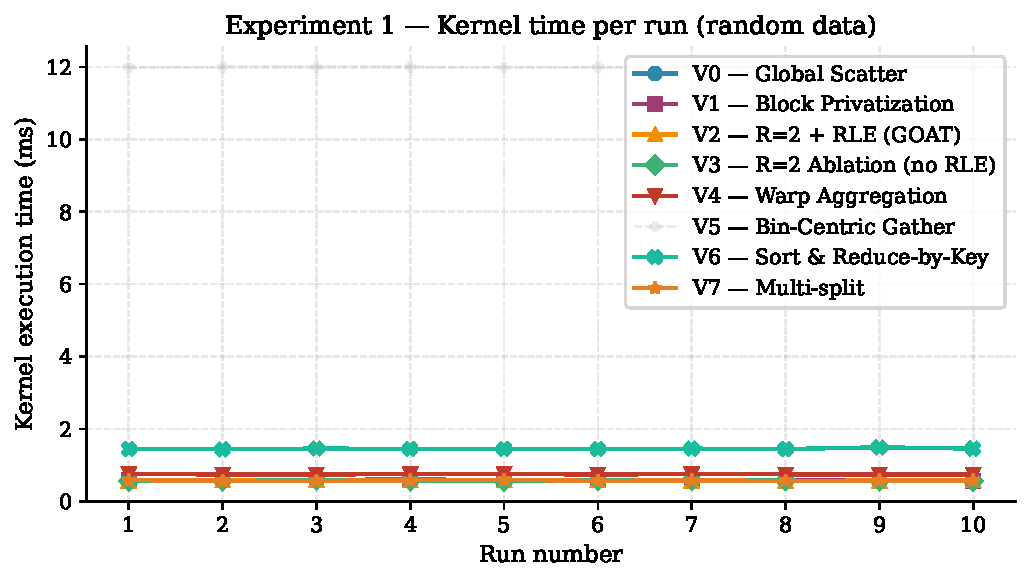
\includegraphics[width=\textwidth]{fig_exp1_runs.pdf}
    \caption{Run-by-run timing}
  \end{subfigure}
  \hfill
  \begin{subfigure}[b]{0.48\textwidth}
    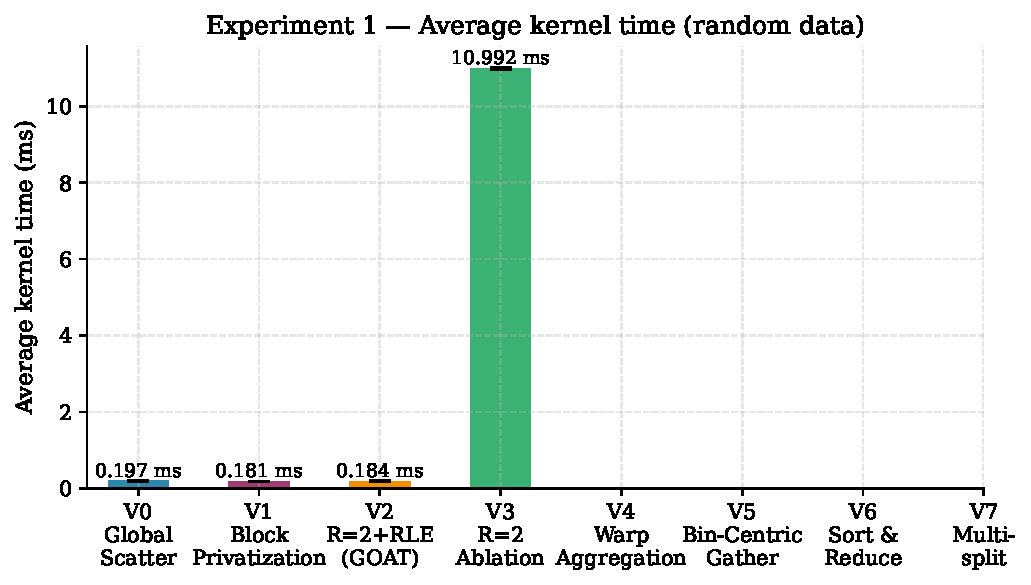
\includegraphics[width=\textwidth]{fig_exp1_bar.pdf}
    \caption{Average with std dev}
  \end{subfigure}
  \caption{Experiment 1 — kernel execution time, random data}
  \label{fig:exp1}
\end{figure}

\begin{figure}[H]
  \centering
  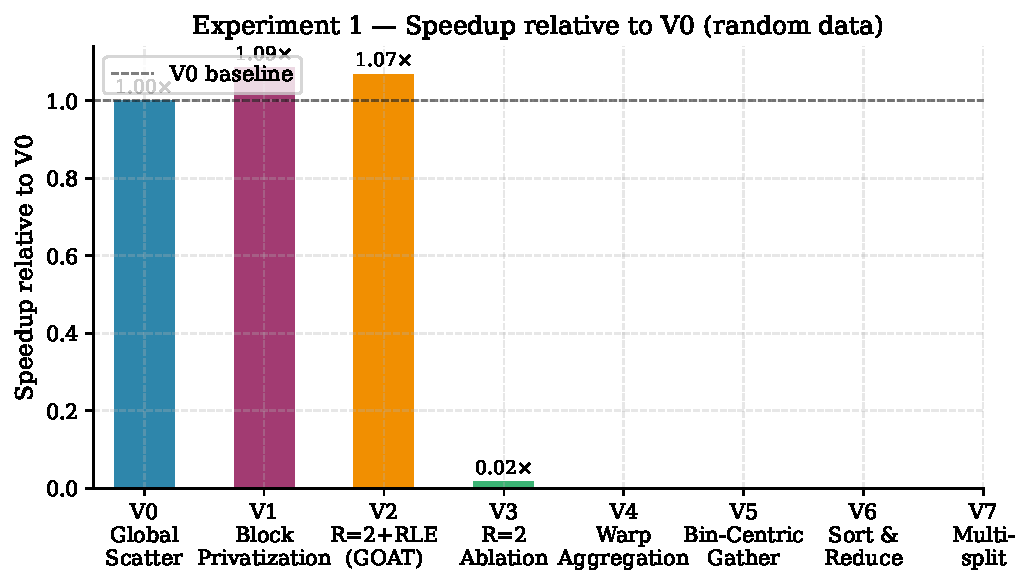
\includegraphics[width=0.55\textwidth]{fig_exp1_speedup.pdf}
  \caption{Experiment 1 — speedup of V1, V2, V3 relative to V0 baseline}
  \label{fig:exp1_speedup}
\end{figure}

% ════════════════════════════════════════════════════════════
\section{Experiment 2: Uniform Data (Same Value)}
% ════════════════════════════════════════════════════════════

The uniform dataset contains 500{,}000 elements all set to the same
value (42), directing all atomic traffic to a single bin.
This stress-tests contention in each implementation.

\begin{table}[H]
\centering
\caption{Kernel execution time — Experiment 2 (uniform, 500k elements, 4096 bins, clipped at 127)}
\label{tab:exp2}
\begin{tabular}{ccccc}
\toprule
\textbf{Run} &
\textbf{V0 (ms)} &
\textbf{V1 (ms)} &
\textbf{V2 (ms)} &
\textbf{V3 (ms)} \\
\midrule
1  & \ETwoVZeroOne   & \ETwoVOneOne   & \ETwoVTwoOne   & \ETwoVThreeOne   \\
2  & \ETwoVZeroTwo   & \ETwoVOneTwo   & \ETwoVTwoTwo   & \ETwoVThreeTwo   \\
3  & \ETwoVZeroThree & \ETwoVOneThree & \ETwoVTwoThree & \ETwoVThreeThree \\
4  & \ETwoVZeroFour  & \ETwoVOneFour  & \ETwoVTwoFour  & \ETwoVThreeFour  \\
5  & \ETwoVZeroFive  & \ETwoVOneFive  & \ETwoVTwoFive  & \ETwoVThreeFive  \\
6  & \ETwoVZeroSix   & \ETwoVOneSix   & \ETwoVTwoSix   & \ETwoVThreeSix   \\
7  & \ETwoVZeroSeven & \ETwoVOneSeven & \ETwoVTwoSeven & \ETwoVThreeSeven \\
8  & \ETwoVZeroEight & \ETwoVOneEight & \ETwoVTwoEight & \ETwoVThreeEight \\
9  & \ETwoVZeroNine  & \ETwoVOneNine  & \ETwoVTwoNine  & \ETwoVThreeNine  \\
10 & \ETwoVZeroTen   & \ETwoVOneTen   & \ETwoVTwoTen   & \ETwoVThreeTen   \\
\midrule
\textbf{Avg}   & \textbf{\ETwoVZeroAvg}   & \textbf{\ETwoVOneAvg}   & \textbf{\ETwoVTwoAvg}   & \textbf{\ETwoVThreeAvg}   \\
\textbf{Stdev} & \textbf{\ETwoVZeroStdev} & \textbf{\ETwoVOneStdev} & \textbf{\ETwoVTwoStdev} & \textbf{\ETwoVThreeStdev} \\
\bottomrule
\end{tabular}
\end{table}

\begin{figure}[H]
  \centering
  \begin{subfigure}[b]{0.48\textwidth}
    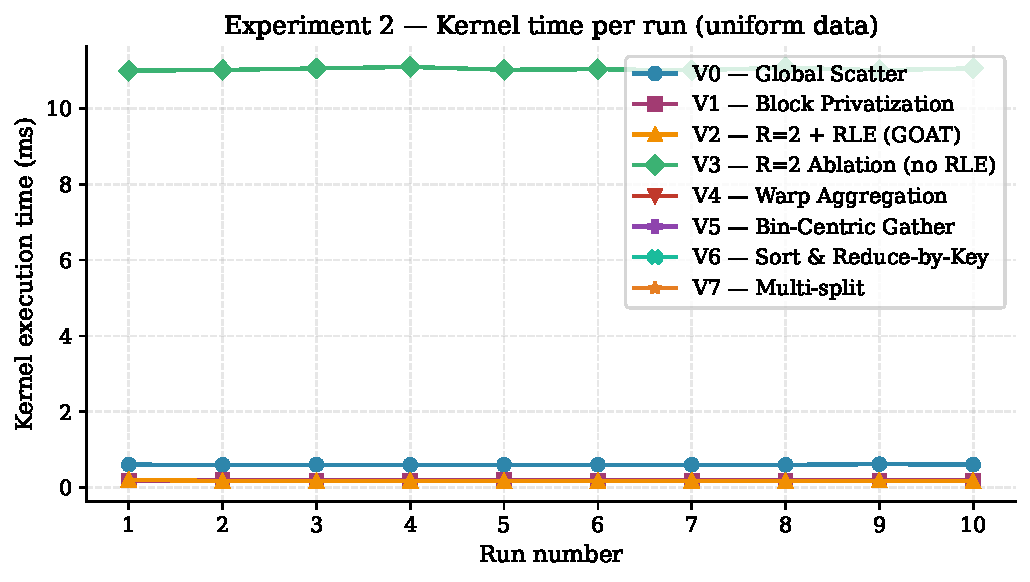
\includegraphics[width=\textwidth]{fig_exp2_runs.pdf}
    \caption{Run-by-run timing}
  \end{subfigure}
  \hfill
  \begin{subfigure}[b]{0.48\textwidth}
    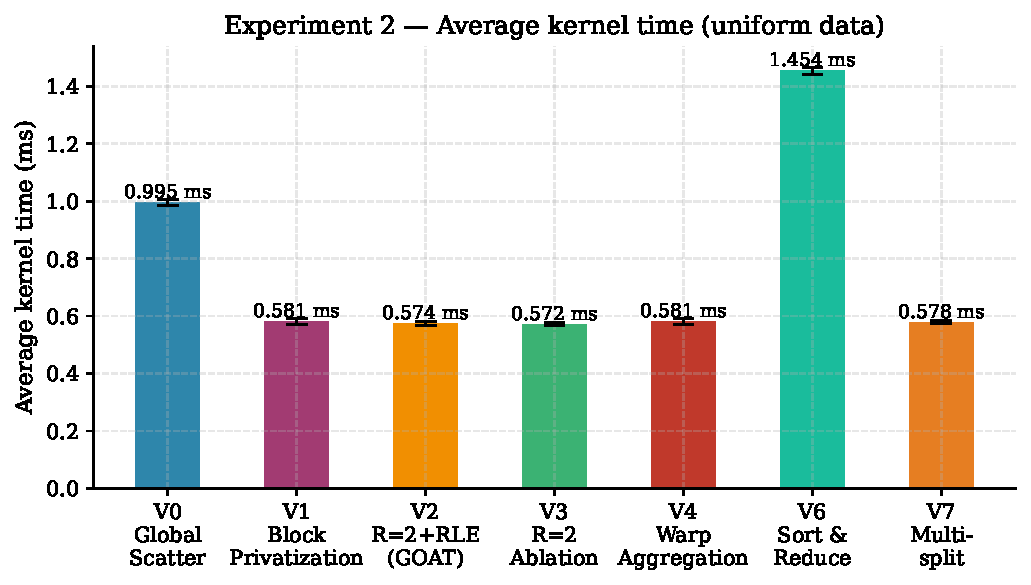
\includegraphics[width=\textwidth]{fig_exp2_bar.pdf}
    \caption{Average with std dev}
  \end{subfigure}
  \caption{Experiment 2 — kernel execution time, uniform data}
  \label{fig:exp2}
\end{figure}

\begin{figure}[H]
  \centering
  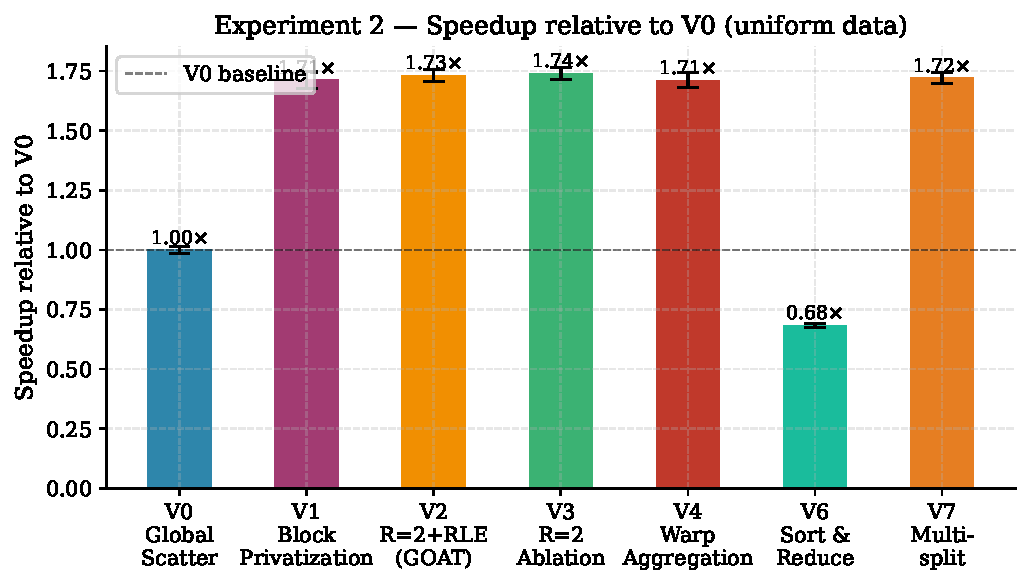
\includegraphics[width=0.55\textwidth]{fig_exp2_speedup.pdf}
  \caption{Experiment 2 — speedup of V1, V2, V3 relative to V0 baseline}
  \label{fig:exp2_speedup}
\end{figure}

\begin{figure}[H]
  \centering
  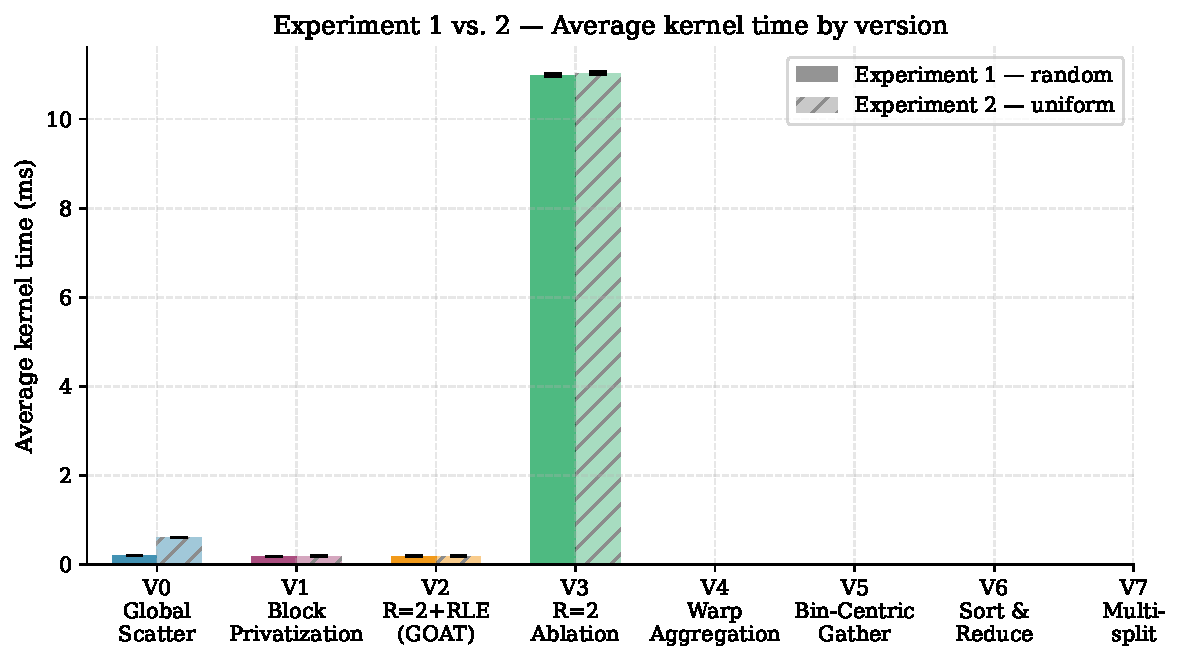
\includegraphics[width=0.65\textwidth]{fig_avg_comparison.pdf}
  \caption{Side-by-side comparison of average kernel time: Experiment 1 vs.\ 2 per version}
  \label{fig:comparison}
\end{figure}

% ════════════════════════════════════════════════════════════
\section{Analysis 1: V0 vs.\ V1 — Global vs.\ Shared Memory}
% ════════════════════════════════════════════════════════════

\subsection*{V0 vs.\ V1 on Experiment 1 (random data)}

[TODO: Compare \EOneVZeroAvg{} ms (V0) vs.\ \EOneVOneAvg{} ms (V1).
Privatization moves atomic operations from global DRAM to on-chip shared
memory.  With random data, 500k elements spread across 4096 bins so each
bin receives $\approx 122$ hits on average and per-bin contention is low.
Compute speedup = $\EOneVZeroAvg / \EOneVOneAvg$ and discuss here.
Reference Figure~\ref{fig:exp1_speedup}.]

\subsection*{V0 vs.\ V1 on Experiment 2 (uniform data)}

[TODO: Compare \ETwoVZeroAvg{} ms (V0) vs.\ \ETwoVOneAvg{} ms (V1).
All elements target bin 42.  V0 serialises every global atomic on one
counter.  V1 serialises within each block's shared copy then merges once
per block to global — far fewer global collisions.
Expected: V1 advantage over V0 is \emph{larger} in Experiment 2 than
Experiment 1.  Reference Figure~\ref{fig:exp2_speedup}.]

\subsection*{Impact of input distribution on V0}

[TODO: Compare \EOneVZeroAvg{} ms (Exp1) vs.\ \ETwoVZeroAvg{} ms (Exp2)
for V0 only.  Random data spreads global atomic pressure across 4096 bins;
uniform data funnels all threads to one bin, maximally serialising the
atomic queue.  Reference Figure~\ref{fig:comparison}.]

\subsection*{Impact of input distribution on V1}

[TODO: Compare \EOneVOneAvg{} ms (Exp1) vs.\ \ETwoVOneAvg{} ms (Exp2)
for V1 only.  Shared atomics are cheaper so the hot-bin penalty is smaller
than in V0.  Expect Exp2 to be only modestly slower than Exp1 for V1,
in contrast to the larger delta seen in V0.  Discuss the ratio.]

% ════════════════════════════════════════════════════════════
\section{Analysis 2: Version 2 — Compression Before Reduction}
% ════════════════════════════════════════════════════════════

\subsection*{Implementation approach}

Version 2 implements the \emph{compression-before-reduction} technique.
Each thread maintains two register variables: \texttt{current\_bin}
(the last bin index encountered) and \texttt{run\_count}
(accumulated hits on that bin).  While consecutive stride elements map to
the same bin, only a register increment fires — zero atomic operations.
On a bin change a single \texttt{atomicAdd} to shared memory flushes the
run.  A final flush handles the trailing run after the loop.
The shared-to-global merge is identical to Version 1.
An additional optimisation pairs this with 128-bit \texttt{uint4} vectorised
loads, quadrupling effective memory bandwidth over V0/V1's 32-bit reads.

Formally let $R_t$ be the number of distinct runs for thread $t$.
V1 issues $N/P$ shared atomics per thread; V2 issues $R_t \leq N/P$.
For fully uniform data $R_t = 1$ regardless of $N$, collapsing the
accumulation phase to a single shared atomic per thread.

\subsection*{Superiority over V0 and V1}

V0 issues one global atomic per element ($N$ total).
V1 replaces these with shared-memory atomics but still issues $N$ total.
V2 reduces the shared-atomic count to $\sum_t R_t$.

For random data runs are length~1 on average, so V2~$\approx$~V1 with
a small constant benefit from the wider loads.  For uniform data V2 yields
$\sum_t R_t = P$ (one atomic per thread), cutting shared atomics by
$N/P - 1$ per thread.

\subsection*{Performance vs.\ data distribution}

\begin{itemize}[noitemsep]
  \item \textbf{Random (Experiment 1):} Minimal run compression; V2
        advantage over V1 is small.  See Figure~\ref{fig:exp1_speedup}.
  \item \textbf{Uniform (Experiment 2):} Maximum compression;
        V2 expected to be significantly faster than V1, and much faster
        than V0.  See Figure~\ref{fig:exp2_speedup}.
  \item \textbf{Skewed data:} Performance lies between the two cases,
        scaling with the degree of skew.
\end{itemize}

[TODO: After data collection, replace the bullet descriptions above with
measured speedup numbers from Tables~\ref{tab:exp1} and~\ref{tab:exp2}
and Figures~\ref{fig:exp1_speedup}--\ref{fig:comparison}.]

% ════════════════════════════════════════════════════════════
\section{Analysis 3: Version 3 — Bin-Centric Gather}
% ════════════════════════════════════════════════════════════

\subsection*{Implementation approach}

Version 3 inverts the scatter pattern used by V0--V2.
Instead of each thread owning an \emph{input element} and scattering it
to a bin, each thread owns a \emph{bin} and scans the input for matches.
With \texttt{num\_bins}=4096 and \texttt{blockDim}=256, exactly 16 blocks
are launched and every bin is covered by exactly one thread.
Because no two threads write to the same bin, \textbf{zero atomic
operations} are needed anywhere.

Shared-memory tiling amortises global memory latency: each block loads a
256-element tile in one coalesced 1024-byte transaction, and all 256 threads
scan the tile simultaneously in registers.

\subsection*{Trade-off}

The elimination of atomics comes at the cost of $O(N \times B)$ comparisons
where $B = 4096$.  For $N = 500{,}000$, each thread performs 500{,}000
comparisons.  This is arithmetic-bound rather than memory-bandwidth-bound.

\subsection*{Expected performance}

\begin{itemize}[noitemsep]
  \item \textbf{Random (Experiment 1):} Moderate — zero atomic overhead
        but high comparison count.
  \item \textbf{Uniform (Experiment 2):} Very Fast — same $O(N \times B)$
        arithmetic, but zero atomic serialisation regardless of how skewed
        the data is.  Unlike V0/V1, performance is distribution-independent.
\end{itemize}

[TODO: Fill in measured times \EOneVThreeAvg{} ms (Exp1)
and \ETwoVThreeAvg{} ms (Exp2) and compare against V0--V2.]

% ════════════════════════════════════════════════════════════
\section{Short Answer Questions}
% ════════════════════════════════════════════════════════════

\subsection*{Global memory reads per kernel}

All kernels (V0--V3) read the input array exactly once — each of the $N$
elements is loaded by exactly one thread on one iteration.
\textbf{Global reads: $N$ for V0, V1, V2, and V3.}

\subsection*{Global memory writes per kernel}

\begin{itemize}[noitemsep]
  \item \textbf{V0:} Every \texttt{atomicAdd(\&bins[b],\,1)} is a global
        read-modify-write.  \textbf{$N$ global atomic writes total.}
  \item \textbf{V1, V2:} Accumulation uses shared memory.  The merge phase
        issues at most $B \times K$ global atomic writes, where $B$ is
        the block count and $K \leq 4096$ is the number of non-zero bins.
        For random data $K = 4096$; for uniform data $K = 1$.
  \item \textbf{V3:} One non-atomic write per bin: exactly 4096 global
        writes total, regardless of $N$ or distribution.
\end{itemize}

\subsection*{Atomic operations per kernel}

\begin{itemize}[noitemsep]
  \item \textbf{V0:} $N$ global atomics — one per element.
  \item \textbf{V1:} $N$ shared atomics (accumulation) $+$ up to
        $B \times K$ global atomics (merge).
        Total: $N + B \cdot K$.
  \item \textbf{V2:} $\sum_t R_t$ shared atomics $+$ up to $B \times K$
        global atomics.  Ranges from $P + B \cdot K$ (uniform) to
        $N + B \cdot K$ (fully random), where $P$ is the total thread count.
  \item \textbf{V3:} \textbf{Zero} — no \texttt{atomicAdd} anywhere.
        Each bin is owned by exactly one thread; no concurrent writes occur.
\end{itemize}

\end{document}
